\begin{figure}
	\centering
	\pgfplotsset{every axis legend/.append style={
		at={(1.05,0.5)},
		anchor=west}}
	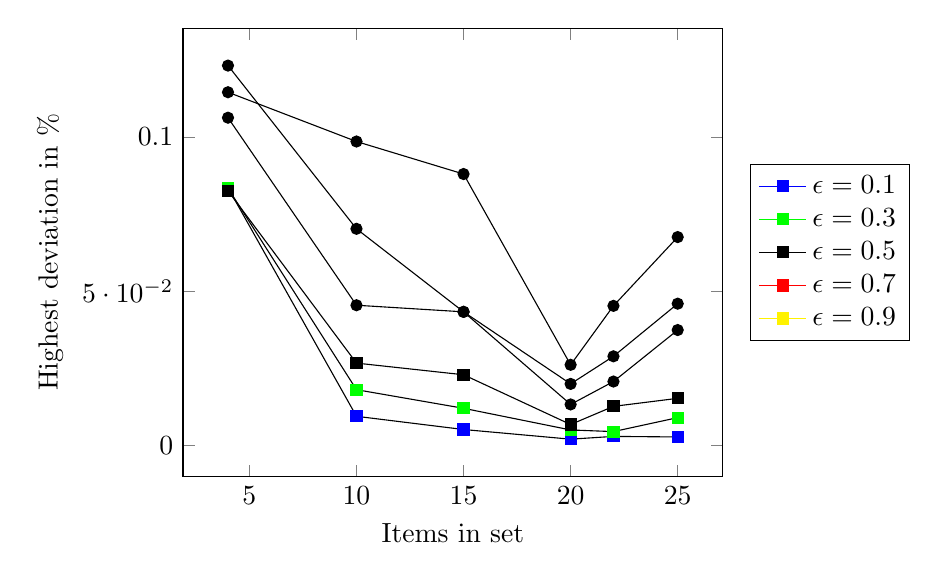
\begin{tikzpicture}
		\begin{axis}[
			xlabel=Items in set,
			ylabel=Highest deviation in \%,
			scatter/classes={
				fptas1={mark=square*,blue},
				fptas3={mark=square*,green},
				fptas5={mark=square*,black},
				fptas7={mark=square*,red},
				fptas9={mark=square*,yellow}
				}
            ]
            
\addplot[scatter,scatter src=explicit symbolic]table[meta=label] {
x y label
4 0.0835 fptas1
10 0.009412 fptas1
15 0.005128 fptas1
20 0.0019934 fptas1
22 0.002894 fptas1
25 0.002714 fptas1
};
\addplot[scatter,scatter src=explicit symbolic]table[meta=label] {
x y label
4 0.08334 fptas3
10 0.01804 fptas3
15 0.012006 fptas3
20 0.004984 fptas3
22 0.00445 fptas3
25 0.008978 fptas3
};
\addplot[scatter,scatter src=explicit symbolic]table[meta=label] {
x y label
4 0.08252 fptas5
10 0.02666 fptas5
15 0.02288 fptas5
20 0.006746 fptas5
22 0.012634 fptas5
25 0.01524 fptas5
};
\addplot[scatter,scatter src=explicit symbolic]table[meta=label] {
x y label
4 0.10622 fptas10
10 0.04542 fptas10
15 0.04328 fptas10
20 0.013262 fptas10
22 0.02068 fptas10
25 0.03738 fptas10
};
\addplot[scatter,scatter src=explicit symbolic]table[meta=label] {
x y label
4 0.12312 fptas15
10 0.0702 fptas15
15 0.04328 fptas15
20 0.019916 fptas15
22 0.02886 fptas15
25 0.04592 fptas15
};
\addplot[scatter,scatter src=explicit symbolic]table[meta=label] {
x y label
4 0.11448 fptas19
10 0.0985 fptas19
15 0.08796 fptas19
20 0.0261 fptas19
22 0.04522 fptas19
25 0.06752 fptas19
};

			\addlegendentry{$\epsilon = 0.1$}
			\addlegendentry{$\epsilon = 0.3$}
			\addlegendentry{$\epsilon = 0.5$}
			\addlegendentry{$\epsilon = 0.7$}
			\addlegendentry{$\epsilon = 0.9$}
		\end{axis}
	\end{tikzpicture}
\caption{Highest deviation for each set of items on normal dataset}
\label{plot:maxDev}
\end{figure}
